\documentclass[11pt,a4paper]{article}
\usepackage[margin=19mm,headheight=15pt]{geometry}
\usepackage[T1]{fontenc}
\usepackage{lmodern}
\usepackage{xcolor,booktabs,tabularx,array,enumitem,fancyhdr,listings,tikz,hyperref}
\usetikzlibrary{arrows.meta,positioning}
\definecolor{ink}{HTML}{183D4B}
\definecolor{accent}{HTML}{375E6A}
\definecolor{pale}{HTML}{F1F4F5}
\definecolor{codekeyword}{HTML}{234B9B}
\definecolor{codestring}{HTML}{8E3534}
\definecolor{codecomment}{HTML}{386A51}
\hypersetup{colorlinks=true,linkcolor=ink,urlcolor=ink,pdftitle={FM School Project Guide}}
\pagestyle{fancy}
\fancyhf{}
\fancyhead[L]{\small FM School}
\fancyhead[R]{\small SEPM Lab \enspace\textbar\enspace Project Guide}
\fancyfoot[C]{\small\thepage}
\renewcommand{\headrulewidth}{0.3pt}
\makeatletter
\renewcommand\section{\@startsection{section}{1}{0pt}{-15pt}{7pt}{\normalfont\Large\bfseries\color{ink}}}
\renewcommand\subsection{\@startsection{subsection}{2}{0pt}{-10pt}{5pt}{\normalfont\large\bfseries\color{ink}}}
\makeatother
\setlength{\parindent}{0pt}
\setlength{\parskip}{5pt}
\setlength{\emergencystretch}{20pt}
\setlist{nosep,leftmargin=1.6em,topsep=4pt,itemsep=3pt}
\renewcommand{\arraystretch}{1.22}
\newcolumntype{Y}{>{\raggedright\arraybackslash}X}
\newcommand{\code}[1]{\texttt{\detokenize{#1}}}
\newcommand{\repo}{https://github.com/FahimHossen121/fm-school-academic}
\lstdefinelanguage{PowerShell}{sensitive=false,morekeywords={git,docker,cd,Set-ExecutionPolicy,Get-Content},morecomment=[l]{\#},morestring=[b]"}
\lstdefinelanguage{JSON}{morekeywords={true,false,null},morestring=[b]"}
\lstdefinelanguage{YAML}{morekeywords={name,on,push,pull_request,workflow_dispatch,permissions,jobs,services,image,env,ports,options,steps,uses,with,run,distribution,cache},morecomment=[l]{\#},morestring=[b]",morestring=[b]'}
\lstset{basicstyle=\small\ttfamily,columns=fullflexible,keepspaces=true,
  showstringspaces=false,breaklines=true,breakatwhitespace=false,
  frame=single,rulecolor=\color{pale},backgroundcolor=\color{pale},
  keywordstyle=\color{codekeyword}\bfseries,stringstyle=\color{codestring},
  commentstyle=\color{codecomment}\itshape,aboveskip=6pt,belowskip=6pt,
  xleftmargin=3pt,xrightmargin=3pt,framesep=4pt}
\lstdefinestyle{source}{basicstyle=\footnotesize\ttfamily,numbers=left,
  numberstyle=\scriptsize\color{accent},numbersep=6pt,xleftmargin=22pt}
\lstdefinestyle{commands}{language=PowerShell}
% Java token colors resolved from the VS Code Light+ theme and Java TextMate grammar.
% VS Code source revision 50bea175f4aa226ab18f45b2837a9112fd2861c8
% Invisible delimiters mark TextMate spans, e.g. (*T00:public:*).
\definecolor{vsBackground}{HTML}{FFFFFF}
\definecolor{vsForeground}{HTML}{000000}
\definecolor{vsGutter}{HTML}{237893}
\definecolor{vsT00}{HTML}{267F99}
\definecolor{vsT01}{HTML}{0000FF}
\definecolor{vsT02}{HTML}{795E26}
\definecolor{vsT03}{HTML}{001080}
\definecolor{vsT04}{HTML}{AF00DB}
\definecolor{vsT05}{HTML}{A31515}
\definecolor{vsT06}{HTML}{098658}
\definecolor{vsT07}{HTML}{008000}
\definecolor{vsT08}{HTML}{EE0000}
\lstdefinestyle{vsJava}{style=source,language={},
  basicstyle=\footnotesize\ttfamily\color{vsForeground},
  backgroundcolor=\color{vsBackground},
  numberstyle=\scriptsize\color{vsGutter},
  moredelim=[is][\color{vsT00}]{(*T00:}{:*)},
  moredelim=[is][\color{vsT01}]{(*T01:}{:*)},
  moredelim=[is][\color{vsT02}]{(*T02:}{:*)},
  moredelim=[is][\color{vsT03}]{(*T03:}{:*)},
  moredelim=[is][\color{vsT04}]{(*T04:}{:*)},
  moredelim=[is][\color{vsT05}]{(*T05:}{:*)},
  moredelim=[is][\color{vsT06}]{(*T06:}{:*)},
  moredelim=[is][\color{vsT07}]{(*T07:}{:*)},
  moredelim=[is][\color{vsT08}]{(*T08:}{:*)},
}

\widowpenalty=10000
\clubpenalty=10000
\begin{document}
{\Huge\bfseries\color{ink} FM School}\par
{\large Project guide for the SEPM lab}\par
Run the application, follow the code, and explain the tests in the viva.
\href{\repo}{GitHub repository}\par
\smallskip
\begin{tabularx}{\linewidth}{@{}Y Y@{}}
\hyperref[sec:setup]{1. Set up and run} & \hyperref[sec:architecture]{2. Understand the code} \\
\hyperref[sec:demo]{3. Demo the main workflows} & \hyperref[sec:api]{4. Use the JSON API} \\
\hyperref[sec:tests]{5. Know the nine new tests} & \hyperref[sec:ci]{6. Run CI and make changes} \\
\hyperref[sec:viva]{7. Prepare for the viva} & \hyperref[sec:code]{8. Application code walkthrough} \\
\hyperref[sec:unitcode]{9. Six unit tests in code} & \hyperref[sec:itcode]{10. Three integration tests in code} \\
\end{tabularx}

\section{Set up and run}\label{sec:setup}
FM School manages Teacher and Student accounts, profiles, course requests, and marks.
The Admin manages records. Teachers and Students work with their own profiles and
enrollments. The project uses Java 25, Spring Boot, Maven, and PostgreSQL 18.6.

\subsection{Start on a Windows lab PC}
Install Git, JDK 25, Docker Desktop, and IntelliJ. Start Docker Desktop and wait
for its engine. Select JDK 25 for the IntelliJ project and Maven importer.
For terminal commands, set \code{JAVA_HOME} to the JDK directory and check
\code{java -version} and \verb|.\mvnw.cmd -version|.
\begin{lstlisting}[style=commands]
git clone https://github.com/FahimHossen121/fm-school-academic.git
cd fm-school-academic
Set-ExecutionPolicy -Scope Process -ExecutionPolicy Bypass
.\run-demo.ps1
\end{lstlisting}
The runner starts PostgreSQL and Spring Boot, applies the demo seed after startup,
and opens \href{http://localhost:8080/login}{localhost:8080/login}.
The seed resets the local Admin password to the demo value. Use it on a lab database.

\begin{tabularx}{\linewidth}{@{}l l Y@{}}
\toprule
Role & Username / password & First page \\
\midrule
Admin & \code{admin} / \code{12345678} & Admin home \\
Teacher & \code{teacher2} / \code{teacher2} & My Profile \\
Student & \code{student2} / \code{student2} & My Profile \\
\bottomrule
\end{tabularx}

\subsection{Run the steps manually if needed}
Start the database with \code{docker compose up -d postgres}. In IntelliJ, run
\code{FmSchoolApplication} and wait for Liquibase to finish. Load the demo rows
from a second terminal and refresh the login page.
\begin{lstlisting}[style=commands]
Get-Content .\demo\seed-demo-data.sql |
  docker compose exec -T postgres psql -v ON_ERROR_STOP=1 -U myuser -d fm_school_db
\end{lstlisting}
Stop Spring Boot with the IDE Stop button if you started it there. If you used
the runner, identify its Java process before stopping it. \code{docker compose stop}
stops PostgreSQL and keeps the volume. GitHub stores code and migrations.
Use the seed to recreate demo data on another PC.

\clearpage
\section{Understand the code}\label{sec:architecture}
A web request enters Spring Security, which checks the user's identity and
route permissions. The controller reads the request. The service applies
business rules. The repository reads or writes the database. The controller
returns an HTML view or JSON.

\begin{center}
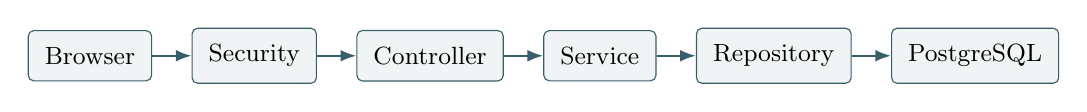
\begin{tikzpicture}[node distance=5mm,
  box/.style={draw=accent,fill=pale,rounded corners=2pt,inner sep=6pt,font=\small},
  arrow/.style={-{Latex[length=2mm]},thick,draw=accent}]
\node[box] (browser) {Browser};
\node[box,right=of browser] (security) {Security};
\node[box,right=of security] (controller) {Controller};
\node[box,right=of controller] (service) {Service};
\node[box,right=of service] (repository) {Repository};
\node[box,right=of repository] (db) {PostgreSQL};
\draw[arrow] (browser) -- (security);
\draw[arrow] (security) -- (controller);
\draw[arrow] (controller) -- (service);
\draw[arrow] (service) -- (repository);
\draw[arrow] (repository) -- (db);
\end{tikzpicture}
\end{center}

\subsection{Find the right file}
Java classes use the package \code{com.example.fmschool}. In IntelliJ, open
files by name with Ctrl+Shift+N.

\begin{tabularx}{\linewidth}{@{}p{.38\linewidth}Y@{}}
\toprule
File or package & Responsibility \\
\midrule
\code{SecurityConfig.java} & Form login, API authentication, role rules, and redirects. \\
\code{StudentController.java} & Admin Student CRUD endpoints and HTTP responses. \\
\code{EnrollmentApiController.java} & API requests to apply, invite, respond, remove, and edit. \\
\code{EnrollmentService.java} & Recipient checks, one accepted course, and Teacher edit authority. \\
\code{ProfileService.java} & Own profile, Admin edits, and account/profile deletion. \\
\code{PeopleApiService.java} & Admin account/profile changes and JSON response DTOs. \\
\code{entity/} and \code{repository/} & Java representations of stored data and the interfaces that query them. \\
\code{dto/} & Data shapes for requests and responses. Validation checks incoming fields. \\
\code{templates/} & Thymeleaf HTML views under \code{src/main/resources/}. \\
\bottomrule
\end{tabularx}

\subsection{The four main tables}
\begin{itemize}
\item \textbf{Accounts} hold the username, role, and password hash.
\item \textbf{Students} hold a name and roll number. \textbf{Teachers} hold a name
and one course. Their account links connect profiles to login identities.
\item \textbf{Enrollments} connect a Student and Teacher. They record who requested
the link, its status, and optional marks. One Student can have several pending
applications and at most one accepted course.
\end{itemize}
Liquibase creates and updates the schema. Its changelog defines the
one-accepted-course constraint and the foreign-key rules for enrollment deletion.
Hibernate validates the schema and maps entities to tables.

\subsection{Follow a profile update}
When a Student submits My Profile, the controller validates the form and calls
\code{ProfileService}. The service looks up the signed-in account, then finds and
saves that account's Student profile. The name and roll belong to the profile.
The username and password hash belong to the account.

\clearpage
\section{Demo the main workflows}\label{sec:demo}
\begin{tabularx}{\linewidth}{@{}l Y@{}}
\toprule
Role & Typical actions \\
\midrule
Admin & Manage Teacher and Student accounts. Directly associate a Student with a Teacher and manage requests. \\
Teacher & Edit own profile, invite Students, respond to applications, and edit names, rolls, and marks for accepted Students. \\
Student & Edit own profile, apply to Teachers, respond to invitations, and view own marks. \\
\bottomrule
\end{tabularx}

\subsection{A quick lab demonstration}
\begin{enumerate}
\item Sign in as \code{teacher2}. Find an accepted Student in the enrollment
board, open the edit page, and enter a mark such as 85.50.
\item Sign out and sign in as that Student. Check the mark on the enrollment
board. Open My Profile to show how the signed-in identity selects the record.
\item To show a pending request, use a new Student and Teacher. Complete both
profiles, then apply as the Student. Sign in as the Teacher and accept. You can
also send an invitation as the Teacher and respond as the Student.
\item Sign in as Admin and open Manage Teachers or Manage Students. Show the
management actions across accounts and profiles.
\end{enumerate}
The seed already enrolls the demo Students. Use a fresh Student account when
demonstrating an application or invitation.

\subsection{Rules to check while demonstrating}
\begin{itemize}
\item The recipient or Admin can accept or reject a pending request. A Teacher
gains edit permission when their enrollment with the Student is accepted.
\item A Student must leave the accepted course before accepting another.
Removing an association leaves both accounts usable.
\item Marks range from 0 to 100 with up to two decimal places. An empty mark
means ungraded. A mark of zero is a grade.
\item A Teacher can edit an accepted Student only through their own enrollment.
Use another Teacher account to demonstrate the denial.
\item Deleting a Teacher account removes the profile and its enrollment links.
The affected Student accounts survive. Use disposable accounts for the demo.
\end{itemize}

\subsection{Troubleshoot the demo}
\begin{tabularx}{\linewidth}{@{}p{.33\linewidth}Y@{}}
\toprule
Symptom & First check \\
\midrule
Database connection error & Run \code{docker compose ps}. Check Docker Desktop and the port mapping in \code{compose.yaml}. \\
Wrong Java version & Check terminal \code{java -version} and IntelliJ's Maven JDK. \\
Demo password rejected & Confirm the app started, then run the demo seed against the local lab database. \\
Port 8080 in use & Identify the process using the port. The runner and IntelliJ can start separate Java processes. \\
Styles look old & Rebuild and refresh. Rebuild Tailwind when changing its input or template classes. \\
\bottomrule
\end{tabularx}

\clearpage
\section{Use the JSON API}\label{sec:api}
The HTML controllers render Thymeleaf pages. The API controllers return JSON
using the same services and ownership rules. A DTO carries selected fields
between the app and the client. Response DTOs leave password hashes out of JSON.

\subsection{Authentication and writes}
Use your browser session or HTTP Basic authentication in Postman. For POST, PUT,
and DELETE, first call \code{GET /api/csrf}. Keep the session cookie and send the
returned token using the returned \code{headerName}. CSRF protection verifies that
a browser write came from a client that obtained the token for that session.

\begin{tabularx}{\linewidth}{@{}p{.55\linewidth}Y@{}}
\toprule
Endpoint & Purpose \\
\midrule
\code{GET /api/session} & See the authenticated username and roles. \\
\code{GET /api/csrf} & Obtain the token and header name. \\
\code{GET}, \code{PUT}, \code{DELETE /api/me} & View, edit, or remove your own Teacher or Student profile and login as applicable. \\
\code{/api/students} and \code{/api/teachers} & Admin lists and creates people. Add an ID to read, update, or delete one record. \\
\code{GET /api/enrollments} & Read the role-filtered board. \\
\code{POST /api/enrollments/applications} & Student applies with a \code{teacherId}. \\
\code{POST /api/enrollments/invitations} & Teacher invites with a \code{studentId}. \\
\code{POST /api/enrollments/associations} & Admin associates a Teacher and Student by profile IDs. \\
\code{POST /api/enrollments/{id}/accept} & Recipient or Admin accepts. Use \code{/reject} to decline. \\
\code{DELETE /api/enrollments/{id}} & Participant removes an accepted link. Admin can remove any link. \\
\code{PUT /api/enrollments/{id}/student} & Associated Teacher or Admin edits Student details and marks on an accepted link. \\
\bottomrule
\end{tabularx}

\subsection{One request to show}
As the associated Teacher, send this JSON to
\code{PUT /api/enrollments/{id}/student}. The enrollment ID identifies the
relationship. You can find it on the enrollment board.
\begin{lstlisting}[language=JSON]
{"name":"Student Two","roll":"9000002","marks":85.50}
\end{lstlisting}
A successful write returns 200. Repeat the call as an unrelated Teacher and
expect 403. When accepting a second course, expect 409 and check that the
original enrollment still exists.

\textbf{Status codes.}
200 success, 201 created, 204 success without a body, 400 invalid input,
401 authentication required, 403 permission or CSRF denied, 404 missing record,
and 409 conflict with the current state.

\clearpage
\section{Know the nine new tests}\label{sec:tests}
A unit test isolates one piece of logic. These six tests call \code{EnrollmentService}
directly and use Mockito repositories. An integration test checks several parts
working together. The three new integration tests use the full Spring application,
MockMvc, Liquibase, and a separate PostgreSQL database. They read the stored results
after HTTP requests complete.

\subsection{Six unit tests}
\begin{tabularx}{\linewidth}{@{}l p{.27\linewidth}Y@{}}
\toprule
& Scenario & What it proves \\
\midrule
U1 & Accept twice & The retry returns 409. The record stays accepted and no second save runs. \\
U2 & Reverse a rejected request & A Teacher invites a Student whose application they rejected. The same row reopens and the Student becomes the recipient. \\
U3 & Filter the invitation list & Students who already have a course or lack a linked account stay out of the picker. \\
U4 & Keep pending history & An enrolled Student still sees pending rows, while the board offers no new Teachers to apply to. \\
U5 & Clear an existing mark & Clearing 78.25 saves a null mark, which means ungraded. \\
U6 & Invite without a profile & A Teacher login without a profile gets a conflict and no enrollment is written. \\
\bottomrule
\end{tabularx}

\subsection{Three integration tests}
\begin{enumerate}
\item \textbf{Transfer courses.} Apply to two Teachers. Accept the first request,
then attempt to accept the second. Check for 409 and confirm the second request
stays pending in PostgreSQL. Remove the first enrollment, accept the second,
and verify there is exactly one accepted row for the Student.
\item \textbf{Roll back a failed creation.} Ask Admin to create a Teacher with
valid account details and no course. The profile step returns 400. Look up the
username in PostgreSQL and verify the earlier account insert was rolled back.
\item \textbf{Delete a Teacher without losing a Student.} Create an accepted
enrollment, delete the Teacher as Admin, and query the database. The Teacher
account, profile, and enrollment are gone. The Student profile survives and the
Student can still sign in with the original credentials.
\end{enumerate}
The existing application startup check also runs in the integration phase.

\subsection{Explain the rollback test in the viva}
The HTTP response tells the client the course is required. Querying the
accounts table shows that the earlier insert was rolled back. A response
assertion alone could pass even if an unused account were left in the database.

\clearpage
\section{Run CI and make changes}\label{sec:ci}

\subsection{Run tests on your PC}
Run unit and isolated web tests with \verb|.\mvnw.cmd test|. To run the integration
tests too, start a disposable PostgreSQL container on port 55432. The demo
database uses port 5432, so both can run independently.
\begin{lstlisting}[style=commands]
docker run -d --rm --name fm-school-lab-test `
  -p 127.0.0.1:55432:5432 `
  -e POSTGRES_DB=fm_school_test -e POSTGRES_USER=fm_school_test `
  -e POSTGRES_PASSWORD=fm_school_test postgres:18.6
docker exec fm-school-lab-test pg_isready -U fm_school_test -d fm_school_test
\end{lstlisting}
Once \code{pg_isready} reports that the database accepts connections, run the
suite and stop the disposable container when finished.
\begin{lstlisting}[style=commands]
.\mvnw.cmd clean verify
docker stop fm-school-lab-test
\end{lstlisting}
The integration profile points to this dedicated database. Maven Surefire
runs \code{*Tests}. Maven Failsafe runs \code{*IT} during \code{verify}.
Reports are in \code{target/surefire-reports} and \code{target/failsafe-reports}.

\subsection{What GitHub Actions does}
The workflow is \code{.github/workflows/tests.yml}. A push or pull request
starts an Ubuntu job. GitHub starts a clean PostgreSQL service, waits for its
health check, sets up Java 25, and executes \code{mvn verify}. Open the
\href{\repo/actions}{Actions tab}, select FM School tests, then open the
\code{verify} job to see the test totals and result.

\subsection{Make a small requested change}
Trace the feature from controller to service before editing. For a marks
range change, check the form, input validation, database constraint, and
boundary tests. Add a new Liquibase changeset when the stored schema changes.

\begin{tabularx}{\linewidth}{@{}p{.28\linewidth}Y@{}}
\toprule
Change & Start here \\
\midrule
Page text or layout & Thymeleaf files in \code{src/main/resources/templates/}. \\
Colors and spacing & Tailwind source in \code{src/main/resources/styles/}. Run \code{npm.cmd ci}, then \code{npm.cmd run css:build}. Commit generated CSS with the source change. \\
Permission or workflow & \code{SecurityConfig} for route rules. The relevant service for record ownership and business rules. \\
Database column & Entity and a new Liquibase changeset. Update DTOs, forms, and tests as needed. \\
\bottomrule
\end{tabularx}
Pull changes before working on a different PC. After editing, run the tests
and review \code{git diff}. Commit the specific files, push, and check the
new Actions run.

\clearpage
\section{Prepare for the viva}\label{sec:viva}

\subsection{How did you create the REST API?}
Open \code{StudentController.java}. Show \code{@RestController},
\code{@RequestMapping("/api/students")}, and \code{@GetMapping}. The GET method
delegates to \code{PeopleApiService.students()}, which queries the repository and
maps results to response DTOs. In the POST method, \code{@RequestBody} binds JSON,
\code{@Valid} checks the request, and creation returns 201 with a Location header.

\subsection{How did you use Docker?}
Open \code{compose.yaml}. PostgreSQL 18.6 runs in Docker, and Spring Boot runs on
the host through IntelliJ or Maven. Compose sets the database name and login,
publishes 5432 to localhost, and attaches \code{postgres_data} to preserve data
across ordinary container recreation. Show \code{docker compose ps}. Explain
that the PostgreSQL driver connects Java to the database.

\subsection{How did you implement Spring Data JPA?}
Show \code{Student.java}, \code{StudentRepository.java}, then
\code{StudentService.updateStudent()}. The entity maps Java fields to columns.
The repository provides methods such as \code{findById} and \code{save}.
The service loads a Student, changes its fields, and saves within a transaction.
Hibernate handles the mapping. Liquibase manages changes to the schema.

\subsection{How did you implement Spring Security?}
Open \code{SecurityConfig.java}. Show the encoder, account lookup through
\code{UserDetailsService}, and the web and API filter chains. A user first proves
who they are. Route rules decide what their role may access. Open
\code{EnrollmentService.requireEditor()} for the record-level check. A Teacher
can edit the Student when the accepted enrollment belongs to that Teacher's
account. The server applies this rule to direct API requests too.

\subsection{What distinguishes the two test types?}
In \code{EnrollmentServiceUnitTests.java}, Mockito supplies the repository
responses and the test checks the service logic. In \code{EnrollmentPersistenceIT.java},
a request passes through security, controller, service, and real database
transactions. Show how the rollback test checks both the response and the
absence of the account in PostgreSQL. Finish by showing the Actions run.

\subsection{Original material}
\begin{itemize}
\item \href{\repo/blob/main/docs/FM\%20School\%20-\%20Complete\%20Project\%20Guide.md}{Full project guide and detailed viva notes}
\item \href{\repo/blob/main/docs/Run\%20on\%20a\%20Fresh\%20PC.md}{Windows lab setup} and
\href{\repo/blob/main/docs/Feature\%20Chunks.md}{feature walkthroughs}
\item \href{\repo/blob/main/docs/JSON\%20API\%20Guide.md}{JSON API reference} and
\href{\repo/blob/main/docs/Styling.md}{Tailwind workflow}
\item \href{\repo/blob/main/docs/Lab\%20Report.md}{REST API, Spring Boot, and Docker lab report}
\end{itemize}
\clearpage
\section{Application code walkthrough}\label{sec:code}
The excerpts keep the repository's line numbers. Click the source label to open
the exact revision. Start with the POST handler below, then follow the service,
database, and security code as needed.

\subsection{Read an HTTP request and create a Student}
A request to \code{POST /api/students} carries login details and a nested Student
profile. The controller turns that request into a call to the application service.

\par\smallskip
{\small\href{\repo/blob/5d22aed7f6d4ef1e4c0b0c0dabf2962ba4b47608/src/main/java/com/example/fmschool/controller/StudentController.java#L31-L35}{\code{StudentController.java}, lines 31--35}}
\begin{lstlisting}[style=source,language=FMJava,firstnumber=31]
@PostMapping
public ResponseEntity<PeopleApiService.StudentView> create(@Valid @RequestBody CreatePersonRequest request) {
    var created = people.createStudent(request);
    return ResponseEntity.created(URI.create("/api/students/" + created.id())).body(created);
}
\end{lstlisting}


\begin{enumerate}
\item \code{@PostMapping} combines with the class path \code{/api/students}.
The request method and path together select this handler.
\item \code{@RequestBody} binds JSON into \code{CreatePersonRequest}.
\code{@Valid} runs field checks before the method executes. The DTO's nested
\code{@Valid} also checks the profile.
\item The controller delegates to \code{people.createStudent(request)}.
The service creates the account and profile, then builds a response view.
\item \code{ResponseEntity.created} returns 201. Its Location header points to
the new Student profile by ID. The response body is the view object.
\end{enumerate}

\par\smallskip
{\small\href{\repo/blob/5d22aed7f6d4ef1e4c0b0c0dabf2962ba4b47608/src/main/java/com/example/fmschool/dto/CreatePersonRequest.java#L6-L11}{\code{CreatePersonRequest.java}, lines 6--11}}
\begin{lstlisting}[style=source,language=FMJava,firstnumber=6]
public record CreatePersonRequest(
        @NotBlank @Size(min = 3, max = 50)
        @Pattern(regexp = "[a-zA-Z0-9._-]+") String username,
        @NotBlank @Size(min = 8, max = 64) String password,
        @NotNull @Valid ProfileForm profile) {
}
\end{lstlisting}

\par\smallskip
{\small\href{\repo/blob/5d22aed7f6d4ef1e4c0b0c0dabf2962ba4b47608/src/main/java/com/example/fmschool/service/PeopleApiService.java#L48-L52}{\code{PeopleApiService.java}, lines 48--52}}
\begin{lstlisting}[style=source,language=FMJava,firstnumber=48]
public StudentView createStudent(CreatePersonRequest request) {
    Long accountId = createIdentity(request, Role.STUDENT);
    profiles.updateManagedProfile(accountId, request.profile());
    return studentView(students.findByAccountId(accountId).orElseThrow());
}
\end{lstlisting}


\textbf{Which ID is which?}
The account ID identifies the login record. The Student profile ID identifies the
row addressed by \code{/api/students/{id}}. The service looks up the profile using
the account ID it just created, then returns the profile view.

\textbf{Follow the GET path.}
The class's list handler calls \code{PeopleApiService.students()}. The service reads
entities with \code{findAll()} and maps each entity to \code{StudentView}. A view
makes the JSON fields explicit, which keeps the password hash out of the response.

\clearpage
\subsection{Map the Student profile and save an update}
An entity represents a database record. The repository provides operations on that
entity. The service decides which record to load and which fields to update.

\par\smallskip
{\small\href{\repo/blob/5d22aed7f6d4ef1e4c0b0c0dabf2962ba4b47608/src/main/java/com/example/fmschool/entity/Student.java#L7-L27}{\code{Student.java}, lines 7--27}}
\begin{lstlisting}[style=source,language=FMJava,firstnumber=7]
@Entity
@Table(name = "students")
public class Student {

    @Id
    @GeneratedValue(strategy = GenerationType.IDENTITY)
    private Long id;

    @Getter
    @Setter
    @com.fasterxml.jackson.annotation.JsonIgnore
    @OneToOne(fetch = FetchType.LAZY)
    @JoinColumn(name = "account_id", unique = true)
    private Account account;

    @Setter
    @Getter
    private String name;
    @Setter
    @Getter
    private String roll;
\end{lstlisting}

\par\smallskip
{\small\href{\repo/blob/5d22aed7f6d4ef1e4c0b0c0dabf2962ba4b47608/src/main/java/com/example/fmschool/repository/StudentRepository.java#L6-L13}{\code{StudentRepository.java}, lines 6--13}}
\begin{lstlisting}[style=source,language=FMJava,firstnumber=6]
public interface StudentRepository extends JpaRepository<Student, Long> {
    java.util.Optional<Student> findByAccountId(Long accountId);

    @org.springframework.data.jpa.repository.Lock(jakarta.persistence.LockModeType.PESSIMISTIC_WRITE)
    @org.springframework.data.jpa.repository.Query("select s from Student s where s.id = :id")
    java.util.Optional<Student> findLockedById(
            @org.springframework.data.repository.query.Param("id") Long id);
}
\end{lstlisting}

\par\smallskip
{\small\href{\repo/blob/5d22aed7f6d4ef1e4c0b0c0dabf2962ba4b47608/src/main/java/com/example/fmschool/service/StudentService.java#L43-L49}{\code{StudentService.java}, lines 43--49}}
\begin{lstlisting}[style=source,language=FMJava,firstnumber=43]
@Transactional
public void updateStudent(Long id, StudentForm form) {
    Student student = getStudentById(id);
    student.setName(form.getName());
    student.setRoll(form.getRoll());
    studentRepository.save(student);
}
\end{lstlisting}


\begin{itemize}
\item \code{@Id} marks the profile's primary key. \code{IDENTITY} lets PostgreSQL
assign the ID. The unique \code{account_id} links at most one Student profile to
the same account. Lazy loading defers fetching that account until needed.
\item \code{JpaRepository<Student, Long>} declares the entity and ID type.
Spring Data provides \code{findById} and \code{save}. It derives
\code{findByAccountId} from the relationship and property names.
\item \code{findLockedById} uses JPQL, which names the Java entity and its
fields. Its pessimistic write lock holds the row until the transaction ends.
That matters for two actions that could try to enroll the same Student.
\item In \code{updateStudent}, a lookup identifies the record, setters change
the in-memory entity, and the save is part of a transaction. The transaction
commits those changes to the database.
\end{itemize}

\clearpage
\subsection{Sign in and choose a landing page}
Authentication answers who the user is. It loads an account by username and
checks the supplied password against the stored hash. The success handler then
chooses the landing page.

\par\smallskip
{\small\href{\repo/blob/5d22aed7f6d4ef1e4c0b0c0dabf2962ba4b47608/src/main/java/com/example/fmschool/config/SecurityConfig.java#L22-L49}{\code{SecurityConfig.java}, lines 22--49}}
\begin{lstlisting}[style=source,language=FMJava,firstnumber=22]
@Bean
public PasswordEncoder passwordEncoder() {
    return PasswordEncoderFactories.createDelegatingPasswordEncoder();
}

@Bean
public UserDetailsService userDetailsService(AccountRepository accounts) {
    return username -> {
        var account = accounts.findByUsername(username)
                .orElseThrow(() -> new UsernameNotFoundException("Account not found"));
        return User.withUsername(account.getUsername())
                .password(account.getPasswordHash())
                .roles(account.getRole().name())
                .build();
    };
}

@Bean
public AuthenticationSuccessHandler roleLoginSuccessHandler() {
    return (request, response, authentication) -> {
        boolean admin = authentication.getAuthorities().stream()
                .anyMatch(a -> a.getAuthority().equals("ROLE_ADMIN"));
        var handler = new SavedRequestAwareAuthenticationSuccessHandler();
        handler.setAlwaysUseDefaultTargetUrl(true);
        handler.setDefaultTargetUrl(admin ? "/" : "/me");
        handler.onAuthenticationSuccess(request, response, authentication);
    };
}
\end{lstlisting}


\begin{enumerate}
\item The encoder supports stored password hashes with an algorithm identifier.
Spring Security uses it to compare passwords during login.
\item \code{UserDetailsService} loads the username, password hash, and role.
A missing account raises \code{UsernameNotFoundException}.
\item \code{roles(...)} gives Spring Security an authority such as
\code{ROLE_TEACHER}. Rules written as \code{hasRole("TEACHER")} check that authority.
\item The success handler checks for \code{ROLE_ADMIN}. It redirects Admin to
\code{/} and Teacher or Student to \code{/me}. The destination comes from the role
Spring loaded from the account.
\end{enumerate}

\textbf{Where the tests touch it.}
Most MockMvc requests set a test identity directly, so they exercise authorization.
The Teacher-deletion integration test goes further by submitting the Student's
real credentials through the form-login filter after deletion.

\clearpage
\subsection{Choose the security rules for a request}
Spring Security uses the first matching filter chain. The API chain has order 1.
The general web chain has order 2.

\par\smallskip
{\small\href{\repo/blob/5d22aed7f6d4ef1e4c0b0c0dabf2962ba4b47608/src/main/java/com/example/fmschool/config/SecurityConfig.java#L51-L86}{\code{SecurityConfig.java}, lines 51--86}}
\begin{lstlisting}[style=source,language=FMJava,firstnumber=51]
@Bean
@Order(2)
public SecurityFilterChain securityFilterChain(HttpSecurity http) throws Exception {
    return http
            .authorizeHttpRequests(auth -> auth
                    .dispatcherTypeMatchers(DispatcherType.ERROR, DispatcherType.FORWARD).permitAll()
                    .requestMatchers("/login", "/signup", "/signup/student", "/signup/teacher",
                            "/css/**", "/favicon.ico").permitAll()
                    .requestMatchers("/students", "/students/**",
                            "/api/students", "/api/students/**",
                            "/admin", "/admin/**").hasRole("ADMIN")
                    .anyRequest().authenticated())
            .formLogin(form -> form.loginPage("/login")
                    .successHandler(roleLoginSuccessHandler()).permitAll())
            .httpBasic(Customizer.withDefaults())
            .logout(logout -> logout.logoutSuccessUrl("/login?logout"))
            .build();
}

@Bean
@Order(1)
public SecurityFilterChain apiFilterChain(HttpSecurity http) throws Exception {
    return http.securityMatcher("/api/**")
            .authorizeHttpRequests(auth -> auth
                    .requestMatchers("/api/students", "/api/students/**",
                            "/api/teachers", "/api/teachers/**").hasRole("ADMIN")
                    .anyRequest().authenticated())
            .httpBasic(basic -> basic.authenticationEntryPoint((request, response, exception) ->
                    apiError(response, 401, "Authentication required")))
            .exceptionHandling(errors -> errors
                    .authenticationEntryPoint((request, response, exception) ->
                            apiError(response, 401, "Authentication required"))
                    .accessDeniedHandler((request, response, exception) ->
                            apiError(response, 403, "Access denied or missing CSRF token")))
            .build();
}
\end{lstlisting}


\begin{itemize}
\item \code{securityMatcher("/api/**")} selects the API chain. The route rules
inside it restrict the people collections to Admin and require authentication for
the other API routes. Basic authentication is available for API clients.
\item The web chain opens login, signup, and static CSS. It protects Admin routes
and configures the form login and logout pages.
\item \code{401} means authentication is required. \code{403} can mean a role or
ownership check failed, or a write lacked a valid CSRF token.
\end{itemize}

A route can permit a Teacher to call an enrollment endpoint. The service must still
check whether the specific enrollment belongs to that Teacher. The next two
sections show that distinction in code.

\clearpage
\subsection{Apply, invite, and respond to an enrollment}
A Student application and a Teacher invitation use the same enrollment table.
\code{requestedBy} records which side sent the request, so the service can identify
the recipient. A rejected pair can reopen through the shared \code{request} method.

\par\smallskip
{\small\href{\repo/blob/5d22aed7f6d4ef1e4c0b0c0dabf2962ba4b47608/src/main/java/com/example/fmschool/service/EnrollmentService.java#L105-L121}{\code{EnrollmentService.java}, lines 105--121}}
\begin{lstlisting}[style=source,language=FMJava,firstnumber=105]
@Transactional
public void respond(Long id, boolean accept) {
    Account actor = currentAccount();
    Enrollment enrollment = enrollment(id);
    // Check who may act before exposing the current request state.
    if (actor.getRole() != Role.ADMIN && !isRecipient(enrollment, actor)) {
        throw forbidden();
    }
    if (enrollment.getStatus() != EnrollmentStatus.PENDING) {
        throw conflict("Only pending requests can be accepted or rejected");
    }
    if (accept) {
        requireAvailable(enrollment.getStudent().getId(), enrollment.getTeacher().getId());
    }
    enrollment.setStatus(accept ? EnrollmentStatus.ACCEPTED : EnrollmentStatus.REJECTED);
    enrollments.save(enrollment);
}
\end{lstlisting}

\par\smallskip
{\small\href{\repo/blob/5d22aed7f6d4ef1e4c0b0c0dabf2962ba4b47608/src/main/java/com/example/fmschool/service/EnrollmentService.java#L136-L153}{\code{EnrollmentService.java}, lines 136--153}}
\begin{lstlisting}[style=source,language=FMJava,firstnumber=136]
private void request(Teacher teacher, Student student, Role sender) {
    student = lockStudent(student.getId());
    requireAvailable(student.getId(), teacher.getId());
    Enrollment enrollment = enrollments.findLockedPair(teacher.getId(), student.getId())
            .orElseGet(Enrollment::new);
    if (enrollment.getStatus() == EnrollmentStatus.ACCEPTED) {
        throw conflict("This Student is already associated with this Teacher");
    }
    if (enrollment.getStatus() == EnrollmentStatus.PENDING) {
        throw conflict("A request is already pending; its recipient must respond");
    }
    // A rejected pair can apply/invite again, without duplicating the association.
    enrollment.setTeacher(teacher);
    enrollment.setStudent(student);
    enrollment.setRequestedBy(sender);
    enrollment.setStatus(EnrollmentStatus.PENDING);
    enrollments.save(enrollment);
}
\end{lstlisting}


\begin{itemize}
\item \code{respond} checks the actor before checking the request status. Only Admin
or the recipient can respond. A second acceptance encounters the status guard
and returns a conflict before the save.
\item Accepting also calls \code{requireAvailable}. It checks whether the Student
already has an accepted enrollment with another Teacher.
\item \code{request} locks the Student and finds the existing Teacher--Student pair.
For a rejected request it reuses the row, sets the new sender, and returns the
status to pending. A pending pair already has a recipient who needs to respond.
\end{itemize}

\textbf{Concurrency.}
\code{enrollment(id)} locks the Student before the enrollment. That serializes
competing acceptances for the same Student. The database also enforces the
one-accepted-course rule through a partial unique index on \code{student_id} for
accepted rows. The course transfer test exercises the rule sequentially.

\clearpage
\subsection{Edit marks through the accepted enrollment}
Teacher edit access depends on the role, the enrollment's status, and the
account that owns the Teacher profile. The service uses the enrollment ID to
load that relationship before writing either record.

\par\smallskip
{\small\href{\repo/blob/5d22aed7f6d4ef1e4c0b0c0dabf2962ba4b47608/src/main/java/com/example/fmschool/service/EnrollmentService.java#L204-L225}{\code{EnrollmentService.java}, lines 204--225}}
\begin{lstlisting}[style=source,language=FMJava,firstnumber=204]
@Transactional
@PreAuthorize("hasAnyRole('TEACHER', 'ADMIN')")
public void updateEnrolledStudent(Long id, @Valid EnrolledStudentForm form) {
    Enrollment enrollment = enrollment(id);
    requireEditor(enrollment, currentAccount());
    Student student = enrollment.getStudent();
    student.setName(form.getName());
    student.setRoll(form.getRoll());
    enrollment.setMarks(form.getMarks());
    students.save(student);
    enrollments.save(enrollment);
    // Account username/password/role are deliberately untouched.
}

private void requireEditor(Enrollment enrollment, Account actor) {
    if (enrollment.getStatus() != EnrollmentStatus.ACCEPTED
            || (actor.getRole() != Role.ADMIN
                && !(actor.getRole() == Role.TEACHER
                    && Objects.equals(enrollment.getTeacher().getAccount().getId(), actor.getId())))) {
        throw forbidden();
    }
}
\end{lstlisting}

\par\smallskip
{\small\href{\repo/blob/5d22aed7f6d4ef1e4c0b0c0dabf2962ba4b47608/src/main/resources/db/changelog/db.changelog-master.yaml#L170-L173}{\code{db.changelog-master.yaml}, lines 170--173}}
\begin{lstlisting}[style=source,language=YAML,firstnumber=170]
    sql: CREATE UNIQUE INDEX enrollments_one_accepted_course ON enrollments (student_id) WHERE status = 'ACCEPTED'
- sql:
    dbms: postgresql
    sql: ALTER TABLE enrollments ADD CONSTRAINT enrollments_marks_range CHECK (marks IS NULL OR (marks >= 0 AND marks <= 100))
\end{lstlisting}


\begin{enumerate}
\item \code{@PreAuthorize} permits Teacher and Admin roles through the method
boundary. \code{requireEditor} requires an accepted enrollment. For Teachers
it compares the enrollment's Teacher account ID with the actor's account ID.
\item The name and roll belong to the Student profile. The mark belongs to the
enrollment, so both are updated within the transaction. Login details stay in
the linked account record.
\item \code{form.getMarks()} can return null. The service stores that null as
ungraded. Zero remains a valid numeric mark. The schema permits null or a
value between 0 and 100.
\end{enumerate}

\textbf{What the board shows.}
\code{getBoard()} gets enrollment rows separately from the lists of people the
user can invite or apply to. That distinction lets a Student see pending history
even when an accepted enrollment hides the new-application picker. A Teacher's
picker filters out Students who already have an accepted course or have no account.

\clearpage
\subsection{Roll back creation and clean up deletions}
The Admin API works across two kinds of records. Account creation writes the
identity first and profile creation fills in the role-specific record afterward.

\par\smallskip
{\small\href{\repo/blob/5d22aed7f6d4ef1e4c0b0c0dabf2962ba4b47608/src/main/java/com/example/fmschool/service/PeopleApiService.java#L13-L16}{\code{PeopleApiService.java}, lines 13--16}}
\begin{lstlisting}[style=source,language=FMJava,firstnumber=13]
@Service
@PreAuthorize("hasRole('ADMIN')")
@Transactional
public class PeopleApiService {
\end{lstlisting}

\par\smallskip
{\small\href{\repo/blob/5d22aed7f6d4ef1e4c0b0c0dabf2962ba4b47608/src/main/java/com/example/fmschool/service/PeopleApiService.java#L78-L82}{\code{PeopleApiService.java}, lines 78--82}}
\begin{lstlisting}[style=source,language=FMJava,firstnumber=78]
public TeacherView createTeacher(CreatePersonRequest request) {
    Long accountId = createIdentity(request, Role.TEACHER);
    profiles.updateManagedProfile(accountId, request.profile());
    return teacherView(teachers.findByAccountId(accountId).orElseThrow());
}
\end{lstlisting}

\par\smallskip
{\small\href{\repo/blob/5d22aed7f6d4ef1e4c0b0c0dabf2962ba4b47608/src/main/java/com/example/fmschool/service/ProfileService.java#L142-L150}{\code{ProfileService.java}, lines 142--150}}
\begin{lstlisting}[style=source,language=FMJava,firstnumber=142]
} else if (account.getRole() == Role.TEACHER) {
    if (form.getCourse() == null || form.getCourse().isBlank()) {
        throw new IllegalArgumentException("Course is required");
    }
    Teacher teacher = teachers.findByAccountId(account.getId()).orElseGet(Teacher::new);
    teacher.setAccount(account);
    teacher.setName(form.getName());
    teacher.setCourse(form.getCourse());
    teachers.save(teacher);
\end{lstlisting}

\par\smallskip
{\small\href{\repo/blob/5d22aed7f6d4ef1e4c0b0c0dabf2962ba4b47608/src/main/java/com/example/fmschool/service/ProfileService.java#L156-L163}{\code{ProfileService.java}, lines 156--163}}
\begin{lstlisting}[style=source,language=FMJava,firstnumber=156]
private void delete(Account account) {
    students.findByAccountId(account.getId()).ifPresent(students::delete);
    teachers.findByAccountId(account.getId()).ifPresent(teachers::delete);
    // Remove dependent records before the account, preserving unrelated people.
    students.flush();
    teachers.flush();
    accounts.delete(account);
}
\end{lstlisting}


\begin{itemize}
\item The class-level \code{@Transactional} on \code{PeopleApiService} gives
\code{createTeacher} a transaction that covers both steps. The nested account
and profile service calls join that transaction.
\item A missing course reaches the Teacher branch of \code{save} and throws an
\code{IllegalArgumentException}. The API handler returns 400. The transaction
rolls back, so the account written by the first step disappears.
\item Deleting an account removes its profiles first and flushes those deletions.
The enrollment foreign keys have \code{ON DELETE CASCADE}, so the linked
enrollment rows disappear when the Teacher profile is deleted.
\item The Student profile belongs to another account. The cascade follows the
deleted Teacher's enrollment links and leaves the Student's login usable.
\end{itemize}

\textbf{What to show in the lab.}
Open integration test I2 for the rollback query and I3 for the row checks plus the
Student's login after the Teacher is gone.

\clearpage
\subsection{Connect the web form and the database}
Thymeleaf renders the profile form with values supplied by Spring MVC. The
browser submits the form to the route shown in the generated HTML.

\par\smallskip
{\small\href{\repo/blob/5d22aed7f6d4ef1e4c0b0c0dabf2962ba4b47608/src/main/resources/templates/profile.html#L27-L51}{\code{profile.html}, lines 27--51}}
\begin{lstlisting}[style=source,language=HTML,firstnumber=27]
<h2>Personal information</h2>
<form
  th:action="@{${savePath}}"
  th:object="${profileForm}"
  method="post"
  class="field-form"
>
  <ul role="alert" th:if="${#fields.hasAnyErrors()}">
    <li
      th:each="error : ${#fields.allErrors()}"
      th:text="${error}"
    ></li>
  </ul>
  <p>
    <label for="name">Name</label>
    <input id="name" type="text" th:field="*{name}" />
  </p>
  <p th:if="${isStudent}">
    <label for="roll">Roll</label>
    <input
      id="roll"
      inputmode="numeric"
      type="text"
      th:field="*{roll}"
    />
\end{lstlisting}


\begin{itemize}
\item \code{th:action} generates the route from the controller's save path.
\code{th:object} selects the profile form object. \code{th:field} connects an
input to one of its fields.
\item The error list displays validation messages after invalid input.
\code{isStudent} selects the Student roll input. The server also validates the
profile before saving it.
\item The shared layout loads the compiled Tailwind stylesheet from
\code{/css/app.css}. Changing Tailwind source requires a CSS build.
\end{itemize}

\par\smallskip
{\small\href{\repo/blob/5d22aed7f6d4ef1e4c0b0c0dabf2962ba4b47608/compose.yaml#L1-L14}{\code{compose.yaml}, lines 1--14}}
\begin{lstlisting}[style=source,language=YAML,firstnumber=1]
services:
  postgres:
    image: 'postgres:18.6'
    environment:
      - 'POSTGRES_DB=fm_school_db'
      - 'POSTGRES_PASSWORD=secret'
      - 'POSTGRES_USER=myuser'
    ports:
      - '127.0.0.1:5432:5432'
    volumes:
      - 'postgres_data:/var/lib/postgresql'

volumes:
  postgres_data:
\end{lstlisting}


The PostgreSQL service publishes its port to localhost. Spring Boot runs on the
host and uses its PostgreSQL driver to reach that port. The named volume keeps
database files across ordinary container recreation.

\clearpage
\subsection{Read the GitHub Actions workflow}
The workflow runs the same Maven verification goal used in local development.
GitHub starts PostgreSQL in a service container on the Ubuntu runner.

\par\smallskip
{\small\href{\repo/blob/5d22aed7f6d4ef1e4c0b0c0dabf2962ba4b47608/.github/workflows/tests.yml#L1-L38}{\code{tests.yml}, lines 1--38}}
\begin{lstlisting}[style=source,language=YAML,firstnumber=1]
name: FM School tests

on:
  push:
  pull_request:
  workflow_dispatch:

permissions:
  contents: read

jobs:
  verify:
    runs-on: ubuntu-latest
    timeout-minutes: 12
    services:
      postgres:
        image: postgres:18.6
        env:
          POSTGRES_DB: fm_school_test
          POSTGRES_USER: fm_school_test
          POSTGRES_PASSWORD: fm_school_test
        ports:
          - 55432:5432
        options: >-
          --health-cmd "pg_isready -U fm_school_test -d fm_school_test"
          --health-interval 5s
          --health-timeout 5s
          --health-retries 12

    steps:
      - uses: actions/checkout@v6
      - uses: actions/setup-java@v5
        with:
          distribution: temurin
          java-version: '25'
          cache: maven
      - name: Run unit and PostgreSQL integration tests
        run: mvn --batch-mode --no-transfer-progress verify
\end{lstlisting}


\begin{enumerate}
\item \code{push} and \code{pull_request} schedule the checks. The workflow also
supports a manual run.
\item The PostgreSQL service waits for \code{pg_isready}. Port 55432 on the runner
maps to port 5432 inside the test database container.
\item Checkout retrieves the repository. Setup Java installs Temurin 25 and
caches Maven dependencies.
\item \code{mvn verify} runs the isolated tests, packages the application,
runs the PostgreSQL tests, and fails the job if either phase reports a failure.
\end{enumerate}

The integration profile uses the same database name and port as this service.
The workflow's successful \code{verify} job is the result to show during the demo.

\clearpage
\section{Six unit tests in code}\label{sec:unitcode}
Each listing contains the complete test method. The fixture code below gives
those methods a Student, a Teacher, and a pending application. The tests call
\code{EnrollmentService} directly.

\subsection{Set up the service and its inputs}
\par\smallskip
{\small\href{\repo/blob/5d22aed7f6d4ef1e4c0b0c0dabf2962ba4b47608/src/test/java/com/example/fmschool/EnrollmentServiceUnitTests.java#L33-L37}{\code{EnrollmentServiceUnitTests.java}, lines 33--37}}
\begin{lstlisting}[style=source,language=FMJava,firstnumber=33]
private final EnrollmentRepository enrollments = mock(EnrollmentRepository.class);
private final AccountRepository accounts = mock(AccountRepository.class);
private final TeacherRepository teachers = mock(TeacherRepository.class);
private final StudentRepository students = mock(StudentRepository.class);
private final EnrollmentService service = new EnrollmentService(enrollments, accounts, teachers, students);
\end{lstlisting}

\par\smallskip
{\small\href{\repo/blob/5d22aed7f6d4ef1e4c0b0c0dabf2962ba4b47608/src/test/java/com/example/fmschool/EnrollmentServiceUnitTests.java#L45-L63}{\code{EnrollmentServiceUnitTests.java}, lines 45--63}}
\begin{lstlisting}[style=source,language=FMJava,firstnumber=45]
@BeforeEach
void setUp() {
    teacherAccount = account(2L, "teacher1", Role.TEACHER);
    studentAccount = account(3L, "student1", Role.STUDENT);
    teacher = new Teacher();
    teacher.setId(10L);
    teacher.setAccount(teacherAccount);
    student = student(20L, "Student One", studentAccount);
    application = enrollment(7L, teacher, EnrollmentStatus.PENDING);

    when(enrollments.findStudentId(7L)).thenReturn(Optional.of(20L));
    when(students.findLockedById(20L)).thenReturn(Optional.of(student));
    when(enrollments.findLockedById(7L)).thenReturn(Optional.of(application));
}

@AfterEach
void clearAuthentication() {
    SecurityContextHolder.clearContext();
}
\end{lstlisting}

\par\smallskip
{\small\href{\repo/blob/5d22aed7f6d4ef1e4c0b0c0dabf2962ba4b47608/src/test/java/com/example/fmschool/EnrollmentServiceUnitTests.java#L159-L169}{\code{EnrollmentServiceUnitTests.java}, lines 159--169}}
\begin{lstlisting}[style=source,language=FMJava,firstnumber=159]
private void signInAs(Account account) {
    when(accounts.findByUsername(account.getUsername())).thenReturn(Optional.of(account));
    SecurityContextHolder.getContext().setAuthentication(new TestingAuthenticationToken(
            account.getUsername(), null, "ROLE_" + account.getRole().name()));
}

private static ResponseStatusException assertStatus(HttpStatus status, Runnable action) {
    var error = assertThrows(ResponseStatusException.class, action::run);
    assertEquals(status, error.getStatusCode());
    return error;
}
\end{lstlisting}


\begin{itemize}
\item The four repository mocks stand in for database calls. The service itself
is the real implementation.
\item \code{setUp()} runs before every test. Teacher account 2 owns Teacher
profile 10. Student account 3 owns Student profile 20. Application 7 connects
them and starts as a request from the Student.
\item The three repository stubs let the service follow application 7 to
Student 20 and load the same application object. Mockito supplies those
values when the service calls the repository.
\item \code{signInAs} sets the test identity and stubs account lookup.
The cleanup method clears the security context after each test.
\end{itemize}

\clearpage
\subsection{U1. An acceptance retry must leave the original result intact}
\par\smallskip
{\small\href{\repo/blob/5d22aed7f6d4ef1e4c0b0c0dabf2962ba4b47608/src/test/java/com/example/fmschool/EnrollmentServiceUnitTests.java#L65-L77}{\code{EnrollmentServiceUnitTests.java}, lines 65--77}}
\begin{lstlisting}[style=source,language=FMJava,firstnumber=65]
@Test
void retryingAcceptanceReturnsConflictWithoutSavingAgain() {
    signInAs(teacherAccount);

    service.respond(7L, true);
    assertEquals(EnrollmentStatus.ACCEPTED, application.getStatus());
    verify(enrollments).save(application);
    clearInvocations(enrollments);

    assertStatus(HttpStatus.CONFLICT, () -> service.respond(7L, true));
    assertEquals(EnrollmentStatus.ACCEPTED, application.getStatus());
    verify(enrollments, never()).save(any());
}
\end{lstlisting}


\begin{enumerate}
\item \textbf{Arrange.} Sign in as the Teacher who received the pending
application. Use the shared application with ID 7.
\item \textbf{Act the first time.} \code{respond(7L, true)} accepts the
application. Check that it is accepted and that the service called
\code{save(application)}.
\item \textbf{Separate the two calls.} \code{clearInvocations} clears Mockito's
recorded calls while keeping its stubs and the accepted application object.
The next verification now measures only the retry.
\item \textbf{Act again and assert.} Expect 409. Check the same record still
says accepted and verify that no repository save followed the retry.
\end{enumerate}

\textbf{Why it matters.}
A user can click twice or retry a request after a slow response. The service
must recognize that the first acceptance already took effect. Checking the
exception alone would miss a second write.

\textbf{Find the production guard.}
In \code{EnrollmentService.respond}, the guard requires \code{PENDING}.
The first call changes the status to \code{ACCEPTED}. The retry stops at the
guard before reaching \code{enrollments.save}.

\clearpage
\subsection{U2. A rejected application can reopen as an invitation}
\par\smallskip
{\small\href{\repo/blob/5d22aed7f6d4ef1e4c0b0c0dabf2962ba4b47608/src/test/java/com/example/fmschool/EnrollmentServiceUnitTests.java#L79-L100}{\code{EnrollmentServiceUnitTests.java}, lines 79--100}}
\begin{lstlisting}[style=source,language=FMJava,firstnumber=79]
@Test
void rejectedApplicationReopensAsInvitationWithStudentAsRecipient() {
    signInAs(teacherAccount);
    service.respond(7L, false);
    assertEquals(EnrollmentStatus.REJECTED, application.getStatus());

    when(teachers.findByAccountId(2L)).thenReturn(Optional.of(teacher));
    when(enrollments.findLockedPair(10L, 20L)).thenReturn(Optional.of(application));
    clearInvocations(enrollments);

    service.invite(20L);

    assertEquals(EnrollmentStatus.PENDING, application.getStatus());
    assertEquals(Role.TEACHER, application.getRequestedBy());
    verify(enrollments).save(same(application));
    assertStatus(HttpStatus.FORBIDDEN, () -> service.respond(7L, true));
    assertEquals(EnrollmentStatus.PENDING, application.getStatus());

    signInAs(studentAccount);
    service.respond(7L, true);
    assertEquals(EnrollmentStatus.ACCEPTED, application.getStatus());
}
\end{lstlisting}


\begin{tabularx}{\linewidth}{@{}p{.23\linewidth}p{.22\linewidth}Y@{}}
\toprule
Action & Stored status & Sender and next actor \\
\midrule
Student applies & Pending & Student sends. Teacher may respond. \\
Teacher rejects & Rejected & A new request can reopen the same pair. \\
Teacher invites & Pending & Teacher sends. Student may respond. \\
Student accepts & Accepted & The association is now active. \\
\bottomrule
\end{tabularx}

\begin{itemize}
\item The Teacher first acts as recipient. After rejecting, the mock returns
the same row for that Teacher--Student pair.
\item \code{verify(...).save(same(application))} checks object identity. This
catches replacing the rejected row with a different object.
\item The invitation changes both the status and \code{requestedBy}. The
Teacher's attempt to accept it now gets 403. The Student then accepts it.
\end{itemize}

\textbf{Viva point.}
The owner of the right to respond changes when the sender changes. Merely
checking for \code{PENDING} would miss that rule.

\clearpage
\subsection{U3. Show only eligible Students in the Teacher's picker}
\par\smallskip
{\small\href{\repo/blob/5d22aed7f6d4ef1e4c0b0c0dabf2962ba4b47608/src/test/java/com/example/fmschool/EnrollmentServiceUnitTests.java#L102-L114}{\code{EnrollmentServiceUnitTests.java}, lines 102--114}}
\begin{lstlisting}[style=source,language=FMJava,firstnumber=102]
@Test
void teacherPickerExcludesOccupiedStudentsAndProfilesWithoutAccounts() {
    signInAs(teacherAccount);
    when(teachers.findByAccountId(2L)).thenReturn(Optional.of(teacher));
    Student occupied = student(21L, "Occupied", account(4L, "occupied", Role.STUDENT));
    Student legacy = student(22L, "Legacy", null);
    when(students.findAll()).thenReturn(List.of(student, occupied, legacy));
    when(enrollments.findStudentIdsByStatus(EnrollmentStatus.ACCEPTED)).thenReturn(List.of(21L));

    var board = service.getBoard();

    assertEquals(List.of(new EnrollmentService.StudentOption(20L, "Student One")), board.students());
}
\end{lstlisting}


The repository returns three Students. The test marks profile 21 as already
enrolled and gives profile 22 no account. Comparing the entire returned list
proves both exclusions and confirms that profile 20 remains selectable.

\subsection{U4. Keep pending rows visible when a Student has a course}
\par\smallskip
{\small\href{\repo/blob/5d22aed7f6d4ef1e4c0b0c0dabf2962ba4b47608/src/test/java/com/example/fmschool/EnrollmentServiceUnitTests.java#L116-L131}{\code{EnrollmentServiceUnitTests.java}, lines 116--131}}
\begin{lstlisting}[style=source,language=FMJava,firstnumber=116]
@Test
void enrolledStudentKeepsPendingRowsButCannotPickANewTeacher() {
    signInAs(studentAccount);
    when(students.findByAccountId(3L)).thenReturn(Optional.of(student));
    Teacher otherTeacher = new Teacher();
    otherTeacher.setId(11L);
    Enrollment accepted = enrollment(8L, otherTeacher, EnrollmentStatus.ACCEPTED);
    when(enrollments.findForAccount(3L)).thenReturn(List.of(application, accepted));
    when(teachers.findAll()).thenReturn(List.of(teacher, otherTeacher));

    var board = service.getBoard();

    assertTrue(board.teachers().isEmpty());
    assertEquals(List.of(7L, 8L), board.rows().stream().map(EnrollmentService.Row::id).toList());
    assertEquals(EnrollmentStatus.PENDING, board.rows().getFirst().status());
}
\end{lstlisting}


The existing accepted row empties the Teacher picker. The two row IDs prove that
the board still shows both relationships, and the status assertion confirms the
older request stays pending.

\textbf{The distinction.}
The picker answers whom the user can apply to now. The rows show existing
requests and enrollments. Filtering the picker should leave that history visible.

\clearpage
\subsection{U5. Clearing a mark returns the enrollment to ungraded}
\par\smallskip
{\small\href{\repo/blob/5d22aed7f6d4ef1e4c0b0c0dabf2962ba4b47608/src/test/java/com/example/fmschool/EnrollmentServiceUnitTests.java#L133-L146}{\code{EnrollmentServiceUnitTests.java}, lines 133--146}}
\begin{lstlisting}[style=source,language=FMJava,firstnumber=133]
@Test
void clearingAnExistingMarkRestoresTheUngradedState() {
    signInAs(teacherAccount);
    application.setStatus(EnrollmentStatus.ACCEPTED);
    application.setMarks(new BigDecimal("78.25"));
    EnrolledStudentForm form = new EnrolledStudentForm();
    form.setName(student.getName());
    form.setRoll(student.getRoll());

    service.updateEnrolledStudent(7L, form);

    assertNull(application.getMarks());
    verify(enrollments).save(application);
}
\end{lstlisting}


The accepted enrollment starts with 78.25. The form keeps the profile fields
and leaves marks unset. The service sets the mark to null and saves the
enrollment. This catches a change that would store zero or retain 78.25.

\subsection{U6. A Teacher without a profile cannot invite}
\par\smallskip
{\small\href{\repo/blob/5d22aed7f6d4ef1e4c0b0c0dabf2962ba4b47608/src/test/java/com/example/fmschool/EnrollmentServiceUnitTests.java#L148-L157}{\code{EnrollmentServiceUnitTests.java}, lines 148--157}}
\begin{lstlisting}[style=source,language=FMJava,firstnumber=148]
@Test
void teacherWithAnAccountButNoProfileCannotSendAnInvitation() {
    signInAs(teacherAccount);
    when(teachers.findByAccountId(2L)).thenReturn(Optional.empty());

    var conflict = assertStatus(HttpStatus.CONFLICT, () -> service.invite(20L));

    assertEquals("Complete My Profile before inviting", conflict.getReason());
    verify(enrollments, never()).save(any());
}
\end{lstlisting}


The account exists and has the Teacher role. \code{findByAccountId(2L)} returns
empty, so the service rejects the invite with the profile-completion message.
\code{never().save(any())} verifies there was no enrollment write.

\textbf{Why check the reason?}
Several enrollment rules can return 409. The reason proves that the missing
profile caused the conflict.

\clearpage
\subsection{Read the fixture helpers}
These builders create plain entity objects. Fixed IDs make the scenarios
readable. The integration tests use database-generated IDs instead.

\par\smallskip
{\small\href{\repo/blob/5d22aed7f6d4ef1e4c0b0c0dabf2962ba4b47608/src/test/java/com/example/fmschool/EnrollmentServiceUnitTests.java#L171-L196}{\code{EnrollmentServiceUnitTests.java}, lines 171--196}}
\begin{lstlisting}[style=source,language=FMJava,firstnumber=171]
private Enrollment enrollment(long id, Teacher assignedTeacher, EnrollmentStatus status) {
    Enrollment enrollment = new Enrollment();
    enrollment.setId(id);
    enrollment.setTeacher(assignedTeacher);
    enrollment.setStudent(student);
    enrollment.setRequestedBy(Role.STUDENT);
    enrollment.setStatus(status);
    return enrollment;
}

private static Account account(long id, String username, Role role) {
    Account account = new Account();
    account.setId(id);
    account.setUsername(username);
    account.setRole(role);
    return account;
}

private static Student student(long id, String name, Account account) {
    Student student = new Student();
    ReflectionTestUtils.setField(student, "id", id);
    student.setName(name);
    student.setRoll("00123");
    student.setAccount(account);
    return student;
}
\end{lstlisting}


\begin{itemize}
\item \code{enrollment} connects the supplied Teacher to the shared Student.
Every fixture starts with the Student as sender unless the test changes it.
\item \code{account} supplies the identity the service will resolve during the
test. The Teacher profile's ID and the Teacher account's ID are separate values.
\item \code{student} sets the generated ID through Spring's test utility because
the production entity has no ID setter. Passing null for the account creates
the legacy profile used by U3.
\end{itemize}

To run just these six tests from Windows PowerShell with JDK 25 configured:
\begin{lstlisting}[style=commands]
.\mvnw.cmd '-Dtest=EnrollmentServiceUnitTests' test
\end{lstlisting}

\clearpage
\section{Three integration tests in code}\label{sec:itcode}

\subsection{Start a real application context and use a test database}
\par\smallskip
{\small\href{\repo/blob/5d22aed7f6d4ef1e4c0b0c0dabf2962ba4b47608/src/test/java/com/example/fmschool/EnrollmentPersistenceIT.java#L24-L35}{\code{EnrollmentPersistenceIT.java}, lines 24--35}}
\begin{lstlisting}[style=source,language=FMJava,firstnumber=24]
@SpringBootTest
@ActiveProfiles("integration")
class EnrollmentPersistenceIT {
    private static final String TEST_PASSWORD = "TestPass123!";
    @Autowired private WebApplicationContext context;
    @Autowired private JdbcTemplate db;
    private MockMvc mvc;

    @BeforeEach
    void setUp() {
        mvc = webAppContextSetup(context).apply(springSecurity()).build();
    }
\end{lstlisting}

\par\smallskip
{\small\href{\repo/blob/5d22aed7f6d4ef1e4c0b0c0dabf2962ba4b47608/src/test/resources/application-integration.properties#L1-L5}{\code{application-integration.properties}, lines 1--5}}
\begin{lstlisting}[style=source,language=YAML,firstnumber=1]
# Use a dedicated database for integration tests. Liquibase builds the schema.
spring.docker.compose.enabled=false
spring.datasource.url=jdbc:postgresql://127.0.0.1:55432/fm_school_test
spring.datasource.username=fm_school_test
spring.datasource.password=fm_school_test
\end{lstlisting}


\begin{enumerate}
\item \code{@SpringBootTest} loads the controllers, security, services,
repositories, and Liquibase.
\item \code{@ActiveProfiles("integration")} selects a dedicated PostgreSQL
database at port 55432. The profile disables the app's usual Compose startup.
The test database is supplied by the local disposable container or GitHub Actions.
\item \code{webAppContextSetup} builds MockMvc from the real application context.
\code{springSecurity()} attaches the filter chain. The request runs inside the
test process.
\item \code{JdbcTemplate} checks stored rows after requests finish. These tests
let service transactions commit or roll back normally so the query can check
what actually persisted.
\end{enumerate}

\textbf{Identity and CSRF.}
\code{with(user(...).roles(...))} supplies the authenticated test identity.
The service still resolves that username against a real account. \code{with(csrf())}
supplies the token needed for a write. I3 also sends a login request with the
stored Student's original password.

\textbf{Where the files run.}
Maven Failsafe finds classes ending in \code{IT} during \code{verify}. The
existing startup check and the three scenarios run in this phase.

\clearpage
\subsection{Create fixtures through the API}
\par\smallskip
{\small\href{\repo/blob/5d22aed7f6d4ef1e4c0b0c0dabf2962ba4b47608/src/test/java/com/example/fmschool/EnrollmentPersistenceIT.java#L98-L126}{\code{EnrollmentPersistenceIT.java}, lines 98--126}}
\begin{lstlisting}[style=source,language=FMJava,firstnumber=98]
private Person createPerson(String collection, String name) throws Exception {
    String username = testUsername();
    String body = """
            {"username":"%s","password":"%s","profile":{"name":"%s","roll":"00123","course":"SEPM"}}
            """.formatted(username, TEST_PASSWORD, name);
    mvc.perform(post("/api/" + collection).with(user("admin").roles("ADMIN")).with(csrf())
                    .contentType("application/json").content(body))
            .andExpect(status().isCreated());
    String query = collection.equals("students")
            ? "select s.id from students s join accounts a on s.account_id = a.id where a.username = ?"
            : "select t.id from teachers t join accounts a on t.account_id = a.id where a.username = ?";
    return new Person(db.queryForObject(query, Long.class, username), username);
}

private long apply(Person student, Person teacher) throws Exception {
    mvc.perform(post("/api/enrollments/applications")
                    .with(user(student.username()).roles("STUDENT")).with(csrf())
                    .contentType("application/json")
                    .content("{\"teacherId\":" + teacher.profileId() + "}"))
            .andExpect(status().isCreated());
    return db.queryForObject("select id from enrollments where student_id = ? and teacher_id = ?",
            Long.class, student.profileId(), teacher.profileId());
}

private void accept(Person teacher, long id, int expectedStatus) throws Exception {
    mvc.perform(post("/api/enrollments/{id}/accept", id)
                    .with(user(teacher.username()).roles("TEACHER")).with(csrf()))
            .andExpect(status().is(expectedStatus));
}
\end{lstlisting}


\begin{itemize}
\item \code{createPerson} posts to the Admin API and expects 201. The test
looks up the new profile ID by joining it to the account's unique username.
\item \code{apply} posts the Teacher profile ID as the Student. The following
query retrieves the new enrollment ID for that pair.
\item \code{accept} calls the enrollment route as the specified Teacher and
checks the expected response. The same helper handles successful and
conflicting attempts.
\end{itemize}

The usernames include UUIDs. This keeps fixture names distinct when tests run
again against the same disposable database.

\clearpage
\subsection{I1. A Student can transfer only after leaving the first course}
\par\smallskip
{\small\href{\repo/blob/5d22aed7f6d4ef1e4c0b0c0dabf2962ba4b47608/src/test/java/com/example/fmschool/EnrollmentPersistenceIT.java#L37-L60}{\code{EnrollmentPersistenceIT.java}, lines 37--60}}
\begin{lstlisting}[style=source,language=FMJava,firstnumber=37]
@Test
void studentCanTransferOnlyAfterLeavingTheAcceptedCourse() throws Exception {
    var student = createPerson("students", "Student");
    var first = createPerson("teachers", "First Teacher");
    var second = createPerson("teachers", "Second Teacher");
    long firstRequest = apply(student, first);
    long secondRequest = apply(student, second);

    accept(first, firstRequest, 200);
    accept(second, secondRequest, 409);

    assertEquals("ACCEPTED", enrollmentStatus(firstRequest));
    assertEquals("PENDING", enrollmentStatus(secondRequest));

    mvc.perform(delete("/api/enrollments/{id}", firstRequest)
                    .with(user(student.username()).roles("STUDENT")).with(csrf()))
            .andExpect(status().isNoContent());
    accept(second, secondRequest, 200);

    assertEquals(0, count("select count(*) from enrollments where id = ?", firstRequest));
    assertEquals("ACCEPTED", enrollmentStatus(secondRequest));
    assertEquals(1, count("select count(*) from enrollments where student_id = ? and status = 'ACCEPTED'",
            student.profileId()));
}
\end{lstlisting}


\begin{enumerate}
\item Create one Student and two Teachers. Submit two applications before
accepting either one. This builds two real pending rows.
\item Accept the first application and expect 200. Accepting the second now
returns 409. Queries confirm the first remains accepted and the second remains
pending.
\item Remove the first enrollment as the Student. Expect 204. The second
acceptance now succeeds because the first association is gone.
\item Check that the old row was deleted, the second row is accepted, and the
Student has exactly one accepted enrollment.
\end{enumerate}

\textbf{What this proves.}
The rule is enforced across separate requests and committed database state. A
failed acceptance leaves the pending row available after the Student leaves
the original course.

\clearpage
\subsection{I2. A failed profile save rolls back the account}
\par\smallskip
{\small\href{\repo/blob/5d22aed7f6d4ef1e4c0b0c0dabf2962ba4b47608/src/test/java/com/example/fmschool/EnrollmentPersistenceIT.java#L62-L75}{\code{EnrollmentPersistenceIT.java}, lines 62--75}}
\begin{lstlisting}[style=source,language=FMJava,firstnumber=62]
@Test
void teacherCreationRollsBackTheAccountWhenCourseIsMissing() throws Exception {
    String username = testUsername();
    String body = """
            {"username":"%s","password":"%s","profile":{"name":"Test Teacher"}}
            """.formatted(username, TEST_PASSWORD);

    mvc.perform(post("/api/teachers").with(user("admin").roles("ADMIN")).with(csrf())
                    .contentType("application/json").content(body))
            .andExpect(status().isBadRequest())
            .andExpect(jsonPath("$.message").value("Course is required"));

    assertEquals(0, count("select count(*) from accounts where username = ?", username));
}
\end{lstlisting}


\begin{enumerate}
\item Build valid account data with a unique username and a valid profile name.
Omit only the course. The request can reach the service's role-specific rule.
\item Post the request as Admin with a CSRF token. Check 400 and the message
\code{Course is required}. That confirms the profile save rejected this request.
\item Query the accounts table by username. A count of zero proves the identity
created earlier in the transaction was rolled back.
\end{enumerate}

\textbf{Walk through the call chain.}
\code{TeacherApiController} invokes \code{PeopleApiService.createTeacher}.
The service creates the identity, then calls \code{updateManagedProfile}.
The missing course throws an exception inside the transaction. PostgreSQL
rolls back the account insert, and the exception handler returns 400.

\textbf{Why query the database?}
A controller could return the expected status even if it left an account
behind. The query detects that partial write.

\clearpage
\subsection{I3. Delete a Teacher and keep the Student's login usable}
\par\smallskip
{\small\href{\repo/blob/5d22aed7f6d4ef1e4c0b0c0dabf2962ba4b47608/src/test/java/com/example/fmschool/EnrollmentPersistenceIT.java#L77-L96}{\code{EnrollmentPersistenceIT.java}, lines 77--96}}
\begin{lstlisting}[style=source,language=FMJava,firstnumber=77]
@Test
void deletingATeacherRemovesTheEnrollmentButStudentCanStillSignIn() throws Exception {
    var student = createPerson("students", "Student");
    var teacher = createPerson("teachers", "Teacher");
    long request = apply(student, teacher);
    accept(teacher, request, 200);
    assertEquals("ACCEPTED", enrollmentStatus(request));

    mvc.perform(delete("/api/teachers/{id}", teacher.profileId())
                    .with(user("admin").roles("ADMIN")).with(csrf()))
            .andExpect(status().isNoContent());

    assertEquals(0, count("select count(*) from accounts where username = ?", teacher.username()));
    assertEquals(0, count("select count(*) from teachers where id = ?", teacher.profileId()));
    assertEquals(0, count("select count(*) from enrollments where id = ?", request));
    assertEquals(1, count("select count(*) from students where id = ?", student.profileId()));
    mvc.perform(formLogin("/login").user(student.username()).password(TEST_PASSWORD))
            .andExpect(authenticated().withUsername(student.username()))
            .andExpect(redirectedUrl("/me"));
}
\end{lstlisting}


\begin{enumerate}
\item Create a Teacher and Student, then accept the application. The initial
database check confirms there is a real accepted enrollment to remove.
\item Delete the Teacher profile through the Admin API. Expect 204.
\item Check that the Teacher's account and profile are gone. Check that the
enrollment is gone too. The Student profile must still exist.
\item Submit the Student's original credentials through form login. Check the
authenticated username and the redirect to \code{/me}.
\end{enumerate}

\textbf{Why test login after deletion?}
The profile query proves the Student row survived. The login proves the linked
account, password hash, and Student role still work through Spring Security.
The test therefore covers both storage and a real user action.

\end{document}
